%=============================================%
%=                                           =%
%=           ..:: STAR BATTLE ::..           =%
%=                                           =%
%=============================================%
%=                                           =%
%=             ..:: Authors ::..             =%
%=                                           =%
%=     Henrique Ferrolho && Joao Pereira     =%
%=                FEUP - 2014                =%
%=                                           =%
%=============================================%

\documentclass[runningheads,a4paper]{llncs}

\usepackage[portuguese]{babel}
\usepackage[utf8]{inputenc}
\usepackage{amssymb}
\setcounter{tocdepth}{3}
\usepackage{graphicx}
\usepackage{url}

\begin{document}

\mainmatter  % start of an individual contribution

\title{Star Battle}
\subtitle{Resolução de Problema de Decisão usando\\
Programação em Lógica com Restrições}
\titlerunning{Star Battle}

\author{Henrique Ferrolho\and João Pereira}
\authorrunning{Henrique Ferrolho\and João Pereira}

\institute{Faculdade de Engenharia da Universidade do Porto\\
Rua Roberto Frias, sn, 4200-465 Porto, Portugal\\}

\toctitle{Star Battle}
\maketitle


\begin{abstract}
Este artigo complementa o segundo projecto da Unidade Curricular de Programação em Lógica, do Mestrado Integrado em Engenharia Informática e de Computação. O projecto consiste num programa, escrito em Prolog, capaz de resolver qualquer tabuleiro do jogo Star Battle, que é um problema de decisão.
\keywords{star battle, sicstus, prolog, feup}
\end{abstract}


\section{Introdução}

O objectivo deste trabalho era implementar a resolução de um problema de decisão ou optimização em Prolog com restrições. Foi dada ao grupo a oportunidade de escolher um dos dois tipos de problema, bem como o puzzle/problema a implementar.

O nosso grupo decidiu implementar o puzzle Star Battle, que é um problema de decisão. O puzzle consiste num tabuleiro quadrado, constituído por diferentes regiões, onde o jogador tem que colocar estrelas.

Este artigo descreve detalhadamente o puzzle Star Battle; a abordagem do grupo para implementar uma resolução capaz de resolver qualquer tabuleiro deste puzzle, bem como a análise detalhada da mesma; a explicação da forma perceptível usada para visualizar qualquer tabuleiro do puzzle e a respectiva solução; estatísticas de resolução de puzzles com diferentes complexidades; e finalmente, a conclusão do projecto realizado.


\section{Descrição do Problema}

O puzzle Star Battle consiste num tabuleiro \textbf{quadrado}, onde existe um dado número de regiões. O número de regiões existentes num dado tabuleiro é \textit{igual ao tamanho desse mesmo tabuleiro}, ou seja, igual ao número de células em cada linha e coluna. As regiões não têm uma forma específica, nem tamanho fixo. 

\begin{figure}
\centering
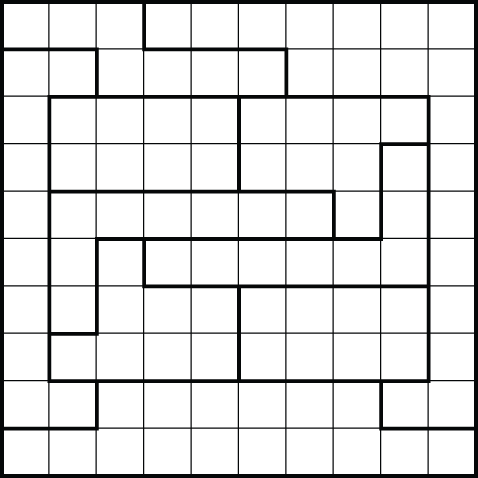
\includegraphics[height=6.2cm]{res/starBattleExample}
\caption{Exemplo de um tabuleiro de Star Battle com dimensões 10x10; e consequentemente, com 10 regiões delimitadas a negrito.}
\label{fig:starBattleExample}
\end{figure}

Juntamente com o tabuleiro é também fornecido um número, que representa o \textbf{número de estrelas} a colocar em cada \textit{linha}, \textit{coluna} e \textit{região} do tabuleiro. A dificuldade do puzzle é consequência do facto de as estrelas \textit{não poderem ser adjacentes umas às outras}, nem sequer diagonalmente.

\begin{figure}
\centering
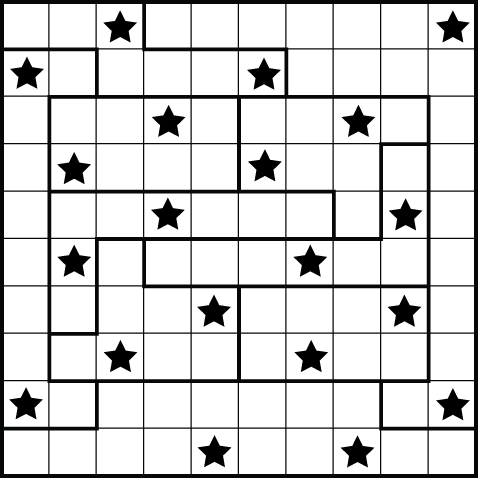
\includegraphics[height=6.2cm]{res/starBattleExampleSolution}
\caption{Solução do tabuleiro apresentado na figura anterior, onde era necessário colocar 2 estrelas em cada linha, coluna e região, sem que nenhuma estrela esteja em contacto com qualquer outra estrela.}
\label{fig:starBattleExampleSolution}
\end{figure}


\section{Abordagem}

Na implementação do puzzle em Prolog, o grupo representou o tabuleiro fornecido como uma \textbf{lista de listas}, onde cada elemento é um número indicador da região a que a célula pertence.

Cada região é identificada por um número único, diferente de todos os outros indicadores das restantes regiões.

\begin{figure}
\centering
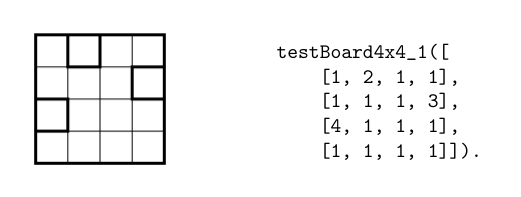
\includegraphics[height=4cm]{res/boardRepresentationExample}
\caption{Um tabuleiro do puzzle Star Battle e a sua respectiva representação na implementação em Prolog do grupo.}
\label{fig:boardRepresentationExample}
\end{figure}


\subsection{Variáveis de Decisão}

Com esta representação em mente, a solução pretendida pode tomar a forma de uma lista simples, com tamanho igual ao do tabuleiro vezes o número de estrelas a colocar em cada linha/coluna/região.

Os primeiros S elementos da solução representam a coluna onde as S estrelas da primeira linha do tabuleiro têm que ser colocadas; os seguintes S elementos, representam a coluna onde as S estrelas da segunda linha têm que ser colocadas; e assim sucessivamente, até à última linha do tabuleiro.

\begin{figure}
\centering
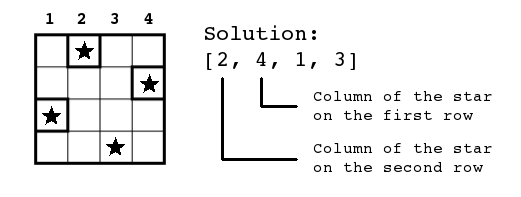
\includegraphics[height=4cm]{res/solutionRepresentationExample}
\caption{A solução de um puzzle Star Battle e a sua respectiva representação na implementação em Prolog do grupo.}
\label{fig:solutionRepresentationExample}
\end{figure}

Sendo \textbf{N} o tamanho do tabuleiro, e \textbf{S} o número de estrelas a colocar em cada \emph{linha/coluna/região}, o \textbf{tamanho da solução} é dado pela expressão:

\begin{equation}
ResultLength = N * S
\end{equation}

O \textbf{domínio} da solução é definido pela dimensão do tabuleiro: uma estrela, para uma dada linha, pode ser colocada desde a coluna \textbf{1}, até à coluna \textbf{N}.

\break

De seguida é apresentado um excerto do predicado de resolução de um tabuleiro, onde se encontram chamadas aos predicados \emph{length} e \emph{domain} relativamente à solução do puzzle.

\begin{verbatim}
solveBoard(Board, S, Result):-
    getBoardSize(Board, N),

    % a board NxN can not have more than N/2 stars
    S #=< (N - 1) // 2 + 1,

    ResultLength #= N * S,
    length(Result, ResultLength),
    domain(Result, 1, N),
    (...)
\end{verbatim}


\subsection{Restrições}

Considera-se novamente - e até ao final deste artigo - que \textbf{N} é o tamanho do tabuleiro, e \textbf{S} o número de estrelas a colocar em cada \emph{linha/coluna/região}.

A resolução do problema pode ser resumida em três restrições:
\begin{enumerate}
  \item Cada coluna deve conter exactamente S estrelas;
  \item Cada região deve conter exactamente S estrelas;
  \item Não pode haver estrelas adjacentes.
\end{enumerate}
Note-se que não está enumerada a restrição: \emph{cada linha deve conter exactamente S estrelas.} Esta regra do puzzle é uma \textbf{consequência} das três restrições acima enumeradas, não havendo necessidade de a implementar também.


\subsubsection{Cada coluna deve conter exactamente S estrelas}
\paragraph{}

Para um tabuleiro de tamanho \textbf{N}, percorrem-se recursivamente as colunas de \textbf{1 a N}, e verifica-se se o número de ocorrências dessa coluna na lista da solução é exactamente igual ao número de estrelas, \textbf{S}.


\subsubsection{Cada região deve conter exactamente S estrelas}
\paragraph{}

Esta restrição é muito semelhante à anterior, na medida em que temos que verificar que, para cada região de \textbf{1 a N}, o número de ocorrências para uma dada região é exactamente igual ao número de estrelas, \textbf{S}.
Para isso, declara-se que existe uma lista adicional, com o mesmo tamanho e domínio da lista da solução, mas que em vez de conter a coluna de cada estrela, em cada linha, contém a região onde cada estrela, em cada linha, está colocada.


\subsubsection{Não pode haver estrelas adjacentes}
\paragraph{}

Finalmente, a terceira e última restrição define que, numa linha, as estrelas têm que estar colocadas a uma distância superior a \textbf{1 unidade} entre elas - isto garante que não há estrelas adjacentes numa linha.

Para garantir que não há estrelas adjacentes entre duas linhas, define-se que para cada estrela de uma determinada linha, esta tem que estar a uma distância superior a \textbf{1 unidade} de qualquer estrela da linha anterior.


\subsubsection{Predicados das restrições}
\paragraph{}

De seguida é apresentada mais uma porção do predicado de resolução do puzzle, onde são chamados os predicados referentes a cada uma das restrições descritas em cima.

\begin{verbatim}
    (...)
    % 1st restriction
    validateNumOfOccurrencesForEachElem(Result, S, N),

    % 2nd restriction
    fetchResultRegions(Board, Result, N, S, ResultRegions),
    validateNumOfOccurrencesForEachElem(ResultRegions, S, N),

    % 3rd restriction
    noAdjacentStars(Result, S, N),
    (...)
\end{verbatim}


\section{Visualização da Solução}

Ao contrário do que se esperava, os predicados responsáveis pela visualização dos possíveis tabuleiros do puzzle em modo de texto, bem como a respectiva solução nesses mesmos tabuleiros, foi a parte mais morosa e trabalhosa deste projecto.

Contudo, o grupo orgulha-se bastante do resultado obtido.

\paragraph{}

\begin{figure}
\centering
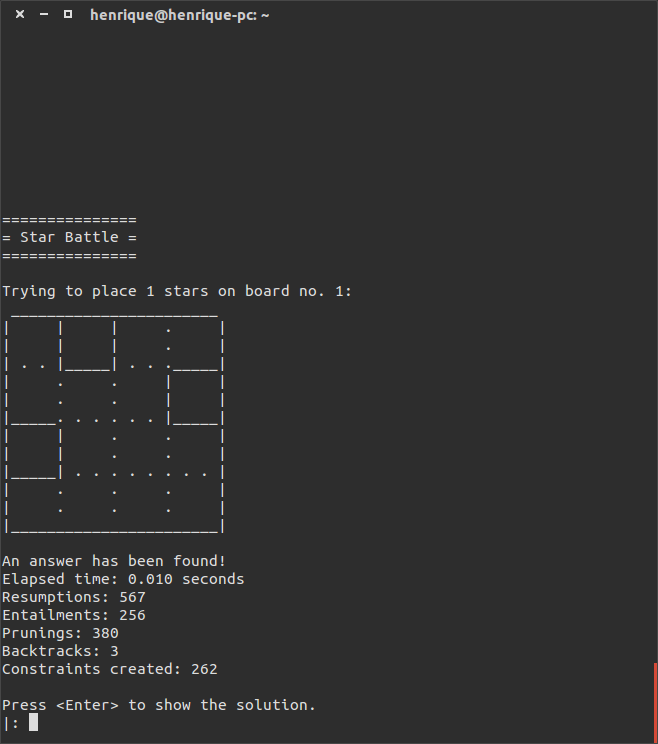
\includegraphics[height=8cm]{res/testBoard4x4_1}
\caption{Representação de um tabuleiro, por resolver, em modo de texto, previamente apresentado noutra imagem.}
\label{fig:testBoard4x4_1}
\end{figure}

\begin{figure}
\centering
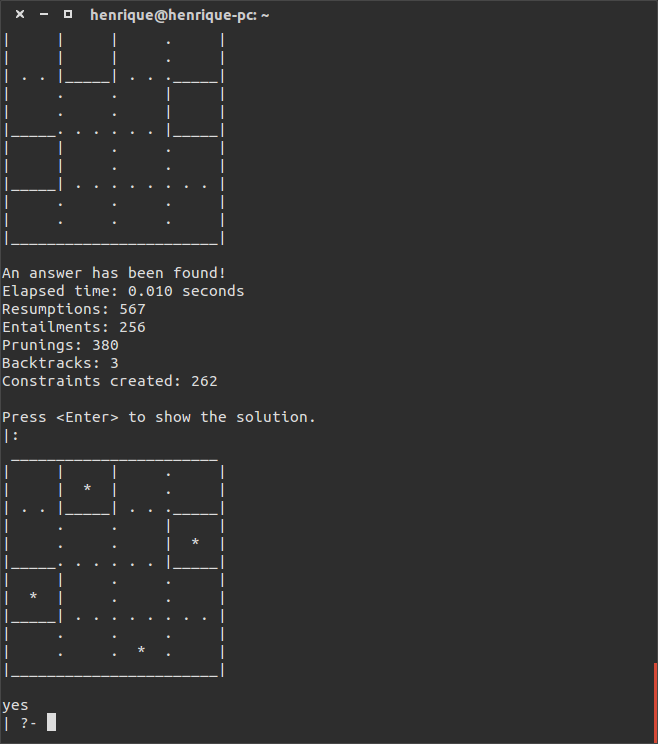
\includegraphics[height=8cm]{res/testBoard4x4_1-solution}
\caption{Representação do tabuleiro da imagem anterior, desta vez preenchido com a solução.}
\label{fig:testBoard4x4_1-solution}
\end{figure}

Os predicados responsáveis pelas representações acima demonstradas encontram-se no ficheiro \emph{printer.pl}.

\paragraph{}

Sucintamente, o que está a acontecer é o seguinte: o tabuleiro está a ser impresso \emph{linha a linha}, e para cada elemento de uma dada linha é verificado o valor da região da célula a \emph{este} e a \emph{sul}; consoante este valor, a célula a ser impressa terá uma \textbf{borda direita} preenchida ou ponteada, se a célula à sua direita pertencer a uma região diferente, ou não, respectivamente, e uma \textbf{borda inferior} preenchida ou ponteada, se a célula a sul pertencer a uma região diferente, ou não, respectivamente.

Os casos especiais das células que se encontram nos limites e nos cantos do tabuleiro são processados devidamente.


\section{Resultados}

Os resultados obtidos não são muito conclusivos porque não foram suficientemente extensos e exaustivos.

Contudo, podem tirar-se as seguintes conclusões:
\begin{itemize}
  \item Colocar uma estrela é extremamente rápido em qualquer um dos tabuleiros testados, sendo o tempo decorrido 0.00 segundos para todos os casos;
  \item Para os tabuleiros onde é possível colocar duas estrelas, na maioria dos casos testados, o tempo necessário para o efeito é inferior a 1 segundo;
  \item Existe um caso que se destacou pelo tempo que o programa demorou a encontrar uma solução, pelo que podemos concluir que houve muitos retrocessos até a solução correcta ter sido encontrada;
  \item O tempo necessário para encontrar a solução de um puzzle aumenta, quer com o número de estrelas a ser colocado, quer com a dimensão do tabuleiro.
\end{itemize}

\begin{figure}
\centering
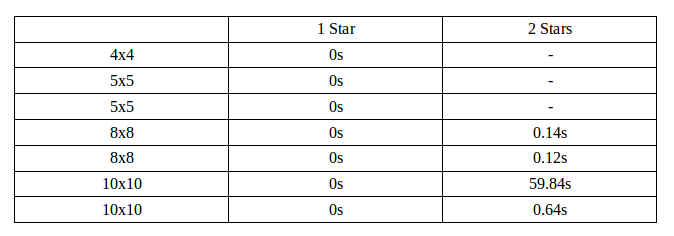
\includegraphics[height=4cm]{res/resultsTable}
\caption{Tempo decorrido para cada tipo de tabuleiro. Células com hífen significam que não há solução para o respectivo número de estrelas, e dimensão do tabuleiro.}
\label{fig:resultsTable}
\end{figure}

\begin{figure}
\centering
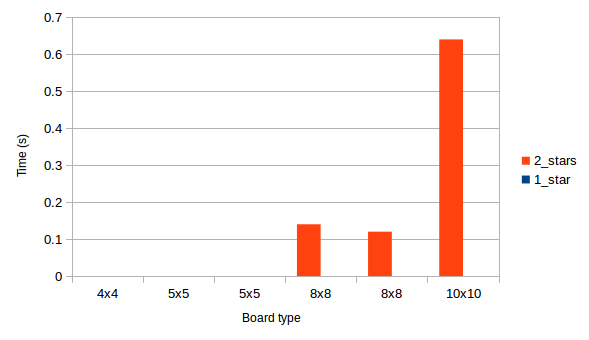
\includegraphics[height=7cm]{res/boardType-timeGraph}
\caption{Gráfico da tabela anterior, ignorando a descrepância do primeiro tabuleiro 10x10.}
\label{fig:boardType-timeGraph}
\end{figure}

\break

\section{Conclusões}

Com a conclusão deste projecto, o grupo conclui que o uso de Prolog com restrições é útil para determinadas situações. O desenvolvimento de programas complexos é facilitado, e dá ao programador a liberdade de escolher o nível de verbosidade que ache mais correcto para os seus predicados.

Por outro lado, uma simples tarefa como imprimir um tabuleiro na consola pode tornar-se facilmente um pesadelo à mínima distração. Se não se tiver cuidado, o tempo ganho ao programar tarefas difíceis que o Prolog descomplica, pode ser gasto e ultrapassado ao programar outras tarefas que o Prolog, talvez, complica.

\paragraph{}

Pudemos também concluir, mais uma vez, que Prolog é uma linguagem bastante eficaz, resolvendo problemas de alguma complexidade bastante rápido.

\begin{thebibliography}{4}

\bibitem{url} Star Battle rules,\\
\url{http://logicmastersindia.com/lmitests/dl.asp?attachmentid=430}

\bibitem{url} SICStus Prolog, \url{https://sicstus.sics.se/}

\bibitem{url} SWI-Prolog, \url{http://www.swi-prolog.org/}

\end{thebibliography}

\pagebreak

\section*{Anexo}

\subsection*{Código fonte}

\newenvironment{changemargin}[2]{%
\begin{list}{}{%
\setlength{\topsep}{0pt}%
\setlength{\leftmargin}{#1}%
\setlength{\rightmargin}{#2}%
\setlength{\listparindent}{\parindent}%
\setlength{\itemindent}{\parindent}%
\setlength{\parsep}{\parskip}%
}%
\item[]}{
\end{list}}

\medskip

\noindent
{\it starBattle.pl}
\begin{changemargin}{-3cm}{-4cm}
\begin{verbatim}

%=============================================%
%=                                           =%
%=           ..:: STAR BATTLE ::..           =%
%=                                           =%
%=        Type 'starBattle.' to start        =%
%=                                           =%
%=============================================%
%=                                           =%
%=             ..:: Authors ::..             =%
%=                                           =%
%=     Henrique Ferrolho && Joao Pereira     =%
%=                FEUP - 2014                =%
%=                                           =%
%=============================================%

%===============%
%= @@ includes =%
%===============%
:- use_module(library(clpfd)).
:- include('containers.pl').
:- include('printer.pl').
:- include('solver.pl').
:- include('starBattleTestBoards.pl').
:- include('utilities.pl').

%====================%
%= @@ game launcher =%
%====================%
starBattle:-
    clearConsole,
    write('To run the program type:'), nl,
    nl,
    write('\tstarBattle(NumBoard, NumStars).'),nl,
    nl,
    write('- NumBoard'), nl,
    write('number of the board you wish to test.'), nl,
    nl,
    write('- NumStars'), nl,
    write('number of stars you wish to place on each row, column and region.'), nl,
    nl.

starBattle(BoardNumber, NumStars):-
    clearConsole,
    write('==============='), nl,
    write('= Star Battle ='), nl,
    write('==============='), nl,
    nl,
    format('Trying to place ~d stars on board no. ~d:', [NumStars, BoardNumber]), nl,

    getBoard(BoardNumber, Board),
    printBoard(Board), !,

    solveBoard(Board, NumStars, Result), !,
    pressEnterToContinue,

    %getBoardSize(Board, BoardSize),
    %printResult(Result, BoardSize, NumStars),
    printResultBoard(Board, Result, NumStars), !.
    
    
\end{verbatim}
\end{changemargin}

\noindent
{\it solver.pl}
\begin{changemargin}{-3cm}{-4cm}
\begin{verbatim}

solveBoard(Board, S, Result):-
    getBoardSize(Board, N),

    % a board NxN can not have more than N/2 stars
    S #=< (N - 1) // 2 + 1,

    ResultLength #= N * S,

    length(Result, ResultLength),
    length(ResultRegions, ResultLength),

    domain(Result, 1, N),
    domain(ResultRegions, 1, N),

    % 1st restriction
    validateNumOfOccurrencesForEachElem(Result, S, N),

    % 2nd restriction
    fetchResultRegions(Board, Result, N, S, ResultRegions),
    validateNumOfOccurrencesForEachElem(ResultRegions, S, N),

    % 3rd restriction
    noAdjacentStars(Result, S, N),

    statistics(walltime, _),
    labeling([bisect], Result),
    statistics(walltime, [_, ElapsedTime | _]),
    format('An answer has been found!~nElapsed time: ~3d seconds', ElapsedTime), nl,
    fd_statistics,
    nl.


%-%-%-%-%-%-%-%-%-%-%-%-%-%-%-%-%-%-%-%-%-%-%-%-%-%-%-%-%-%-%-%-%-%-%

getBoardSize([Head|_], N):-
    length(Head, N).


%-%-%-%-%-%-%-%-%-%-%-%-%-%-%-%-%-%-%-%-%-%-%-%-%-%-%-%-%-%-%-%-%-%-%

validateNumOfOccurrencesForEachElem(Elements, NumOfOccurrences, N):-
    validateNumOfOccurrencesForEachElem(Elements, NumOfOccurrences, N, 1).

validateNumOfOccurrencesForEachElem(Result, S, N, N):-
    exactly(N, Result, S).
validateNumOfOccurrencesForEachElem(Result, S, N, I):-
    exactly(I, Result, S),
    I1 #= I + 1,
    validateNumOfOccurrencesForEachElem(Result, S, N, I1).


%-%-%-%-%-%-%-%-%-%-%-%-%-%-%-%-%-%-%-%-%-%-%-%-%-%-%-%-%-%-%-%-%-%-%

fetchResultRegions(Board, Result, ResRows, ResCols, ResultRegions):-
    fetchResultRegions(Board, Result, ResRows, ResCols, [], 1, ResultRegions).

fetchResultRegions(_, _, ResRows, ResCols, ResultRegions, Pos, ResultRegions):-
    Pos #= ResRows * ResCols + 1.
fetchResultRegions(Board, Result, ResRows, ResCols, ResultRegionsSoFar, Pos, ResultRegions):-
    % calculating row and col of result to access
    Row #= (Pos - 1) // ResCols + 1,
    Col #= ((Pos - 1) mod ResCols) + 1,

    % get the value of result[Row][Col], which is the column where a star is placed
    getMatrixOfListElemAt(Result, ResRows, ResCols, Row, Col, StarCol),

    % get line Row of the board
    getListElemAt(Board, Row, Line),

    % get the region of that position - board[Row][StarCol]
    element(StarCol, Line, Region),

    % push value to ResultRegionsSoFar
    listPushBack(ResultRegionsSoFar, Region, NewResultRegionsSoFar),

    % fetch next element
    Pos1 #= Pos + 1,
    fetchResultRegions(Board, Result, ResRows, ResCols, NewResultRegionsSoFar, Pos1, ResultRegions).


%-%-%-%-%-%-%-%-%-%-%-%-%-%-%-%-%-%-%-%-%-%-%-%-%-%-%-%-%-%-%-%-%-%-%

noAdjacentStars(Result, S, N):-
    noAdjacentStars(Result, S, N, 1).

noAdjacentStars(Result, S, N, 1):-
    noAdjacentStarsOnRow(Result, S, 1),
    noAdjacentStars(Result, S, N, 2).
noAdjacentStars(_, _, N, Row):-
    Row #= N + 1.
noAdjacentStars(Result, S, N, Row):-
    Row #> 1,
    noAdjacentStarsOnRow(Result, S, Row),
    noAdjacentStarsWithPreviousRow(Result, S, Row),
    Row1 #= Row + 1,
    noAdjacentStars(Result, S, N, Row1).


%-%-%-%-%-%-%-%-%-%-%-%-%-%-%-%-%-%-%-%-%-%-%-%-%-%-%-%-%-%-%-%-%-%-%

noAdjacentStarsOnRow(Result, S, Row):-
    StartPos #= (Row - 1) * S + 1,
    EndPos #= StartPos + S,
    validateStarsFromStartToEnd(Result, StartPos, EndPos).

validateStarsFromStartToEnd(Result, Start, End):-
    Next #= Start + 1,
    validateStarsFromStartToEnd(Result, Start, Next, End).

validateStarsFromStartToEnd(_, Start, _, End):-
    Start #= End - 1.
validateStarsFromStartToEnd(Result, Start, End, End):-
    Start1 #= Start + 1,
    Next #= Start1 + 1,
    validateStarsFromStartToEnd(Result, Start1, Next, End).
validateStarsFromStartToEnd(Result, Start, Next, End):-
    validateHorizontalDistanceBetweenStars(Result, Start, Next),
    Next1 #= Next + 1,
    validateStarsFromStartToEnd(Result, Start, Next1, End).


%-%-%-%-%-%-%-%-%-%-%-%-%-%-%-%-%-%-%-%-%-%-%-%-%-%-%-%-%-%-%-%-%-%-%

noAdjacentStarsWithPreviousRow(Result, S, Row):-
    StartPos #= (Row - 1) * S + 1,
    EndPos #= StartPos + S,
    noAdjacentStarsWithPreviousRow(Result, S, Row, StartPos, EndPos).

noAdjacentStarsWithPreviousRow(_, _, _, EndPos, EndPos).
noAdjacentStarsWithPreviousRow(Result, S, Row, CurrentPos, EndPos):-
    % for each star of the row being validated,
    % validate horizontal distance to each star of the previous row
    PrevRow #= Row - 1,
    starIsNotAdjacentWithAnyOfThePreviousRow(Result, S, CurrentPos, PrevRow),
    % procceed to next row
    CurrentPos1 #= CurrentPos + 1,
    noAdjacentStarsWithPreviousRow(Result, S, Row, CurrentPos1, EndPos).

starIsNotAdjacentWithAnyOfThePreviousRow(Result, S, PivotStar, PrevRow):-
    FirstStarPos #= (PrevRow - 1) * S + 1,
    LastStarPos #= FirstStarPos + S,
    starIsNotAdjacentToAnyOtherStarFromFirstToLastPos(Result, PivotStar, FirstStarPos, LastStarPos).

starIsNotAdjacentToAnyOtherStarFromFirstToLastPos(_, _, LastStarPos, LastStarPos).
starIsNotAdjacentToAnyOtherStarFromFirstToLastPos(Result, PivotStar, CurrentStarPos, LastStarPos):-
    validateHorizontalDistanceBetweenStars(Result, PivotStar, CurrentStarPos),
    NextStarPos #= CurrentStarPos + 1,
    starIsNotAdjacentToAnyOtherStarFromFirstToLastPos(Result, PivotStar, NextStarPos, LastStarPos).


%-%-%-%-%-%-%-%-%-%-%-%-%-%-%-%-%-%-%-%-%-%-%-%-%-%-%-%-%-%-%-%-%-%-%

validateHorizontalDistanceBetweenStars(Result, Pos1, Pos2):-
    element(Pos1, Result, Col1),
    element(Pos2, Result, Col2),
    Dist #= abs(Col2 - Col1),
    Dist #> 1.
    
    
\end{verbatim}
\end{changemargin}

\noindent
{\it printer.pl}
\begin{changemargin}{-3cm}{-4cm}
\begin{verbatim}

%===============================%
%= @@ board printing functions =%
%===============================%
printBoard(Board):-
    getBoardSize(Board, N),
    printBoardTopBorder(N),
    printBoard(Board, 1, N),
    nl, !.
printResultBoard(Board, Result, S):-
    getBoardSize(Board, N),
    printBoardTopBorder(N),
    printBoard(Board, 1, N, Result, S),
    nl, !.

printBoardTopBorder(N):-
    N1 is N - 1, createSeparatorN(N1, '______', TopBorder),
    write(' '), printList(TopBorder), write('_____'), nl.

printBoard(Board, N, N):-
    printBoardRow(Board, N, N).
printBoard(Board, I, N):-
    printBoardRow(Board, I, N), !,
    I1 is I + 1,
    printBoard(Board, I1, N).
%-%-%-%-%-%-%
printBoard(Board, N, N, Result, S):-
    printBoardRow(Board, N, N, Result, S).
printBoard(Board, I, N, Result, S):-
    printBoardRow(Board, I, N, Result, S), !,
    I1 is I + 1,
    printBoard(Board, I1, N, Result, S).

%-%-%-%-%-%-%-%-%-%-%-%-%-%-%-%-%-%-%-%-%-%-%-%-%-%-%-%-%-%-%-%-%-%-%

printBoardRow(Board, N, N):-
    write('|'), printBoardRowTop(Board, N, N, 1), nl, !,
    write('|'), printBoardRowMiddle(Board, N, N, 1), nl, !,
    write('|'), printBoardLastRowBottom(Board, N, N, 1), nl, !.
printBoardRow(Board, I, N):-
    write('|'), printBoardRowTop(Board, I, N, 1), nl, !,
    write('|'), printBoardRowMiddle(Board, I, N, 1), nl, !,
    write('|'), printBoardRowBottom(Board, I, N, 1), nl, !.
%-%-%-%-%-%-%
printBoardRow(Board, N, N, Result, S):-
    write('|'), printBoardRowTop(Board, N, N, 1), nl, !,
    write('|'), printBoardRowMiddle(Board, N, N, 1, Result, S), nl, !,
    write('|'), printBoardLastRowBottom(Board, N, N, 1), nl, !.
printBoardRow(Board, I, N, Result, S):-
    write('|'), printBoardRowTop(Board, I, N, 1), nl, !,
    write('|'), printBoardRowMiddle(Board, I, N, 1, Result, S), nl, !,
    write('|'), printBoardRowBottom(Board, I, N, 1), nl, !.

%-%-%-%-%-%-%-%-%-%-%-%-%-%-%-%-%-%-%-%-%-%-%-%-%-%-%-%-%-%-%-%-%-%-%

printBoardRowTop(_, _, N, N):-
    write('     |').
printBoardRowTop(Board, I, N, Col):-
    getListElemAt(Board, I, Row),
    Col1 is Col + 1,
    element(Col, Row, V1),
    element(Col1, Row, V2),
    printCellTop(V1, V2),
    printBoardRowTop(Board, I, N, Col1).

% @@@ swap comment to toggle region display
%printBoardRowMiddle(Board, I, N, N):-
%   getListElemAt(Board, I, Row),
%   element(N, Row, V1),
%   write('  '), write(V1), write('  |').
printBoardRowMiddle(_, _, N, N):-
    write('     |').
printBoardRowMiddle(Board, I, N, Col):-
    getListElemAt(Board, I, Row),
    Col1 is Col + 1,
    element(Col, Row, V1),
    element(Col1, Row, V2),
    printValue(V1, V2),
    printBoardRowMiddle(Board, I, N, Col1).
%-%-%-%-%-%-%
printBoardRowMiddle(_, I, N, N, Result, S):-
    starExistsIn(Result, S, I, N),
    write('  *  |').
printBoardRowMiddle(_, _, N, N, _, _):-
    write('     |').
printBoardRowMiddle(Board, I, N, Col, Result, S):-
    starExistsIn(Result, S, I, Col),

    getListElemAt(Board, I, Row),
    Col1 is Col + 1,
    element(Col, Row, V1),
    element(Col1, Row, V2),
    printStar(V1, V2),
    printBoardRowMiddle(Board, I, N, Col1, Result, S).
printBoardRowMiddle(Board, I, N, Col, Result, S):-
    getListElemAt(Board, I, Row),
    Col1 is Col + 1,
    element(Col, Row, V1),
    element(Col1, Row, V2),
    printValue(V1, V2),
    printBoardRowMiddle(Board, I, N, Col1, Result, S).

printBoardRowBottom(Board, I, N, N):-
    getListElemAt(Board, I, Row),
    I1 is I + 1, getListElemAt(Board, I1, NextRow),

    element(N, Row, V1),
    element(N, NextRow, V3),

    printCellBottom(V1, V3).
printBoardRowBottom(Board, I, N, Col):-
    getListElemAt(Board, I, Row),
    I1 is I + 1, getListElemAt(Board, I1, NextRow),
    NextCol is Col + 1,

    element(Col, Row, V1),
    element(NextCol, Row, V2),
    element(Col, NextRow, V3),

    printCellBottom(V1, V2, V3),
    printBoardRowBottom(Board, I, N, NextCol).

printBoardLastRowBottom(_, _, N, N):-
    write('_____|').
printBoardLastRowBottom(Board, I, N, Col):-
    getListElemAt(Board, I, Row),
    NextCol is Col + 1,

    element(Col, Row, V1),
    element(NextCol, Row, V2),

    printLastRowCellBottom(V1, V2),
    printBoardLastRowBottom(Board, I, N, NextCol).

%-%-%-%-%-%-%-%-%-%-%-%-%-%-%-%-%-%-%-%-%-%-%-%-%-%-%-%-%-%-%-%-%-%-%

printCellTop(V1, V1):-
    write('     .').
printCellTop(_, _):-
    write('     |').

% @@@ swap comment to toggle region display
%printValue(V, V):-
%   write('  '), write(V), write('  .').
printValue(V, V):-
    write('     .').

% @@@ swap comment to toggle region display
%printValue(V, _):-
%   write('  '), write(V), write('  |').
printValue(_, _):-
    write('     |').

printStar(V, V):-
    write('  *  .').
printStar(_, _):-
    write('  *  |').

printCellBottom(V, V, V):-
    write(' . . .').
printCellBottom(V, V, _):-
    write('_____.').
printCellBottom(V, _, V):-
    write(' . . |').
printCellBottom(_, _, _):-
    write('_____|').

printCellBottom(V, V):-
    write(' . . |').
printCellBottom(_, _):-
    write('_____|').

printLastRowCellBottom(V, V):-
    write('______').
printLastRowCellBottom(_, _):-
    write('_____|').


%-%-%-%-%-%-%-%-%-%-%-%-%-%-%-%-%-%-%-%-%-%-%-%-%-%-%-%-%-%-%-%-%-%-%

createSeparatorN(0, _, []).
createSeparatorN(N, SS, [SS | Ls]):-
    N1 is N-1,
    createSeparatorN(N1, SS, Ls).


%-%-%-%-%-%-%-%-%-%-%-%-%-%-%-%-%-%-%-%-%-%-%-%-%-%-%-%-%-%-%-%-%-%-%

starExistsIn(Result, S, Row, StarCol):-
    StartPos is (Row - 1) * S + 1,
    EndPos is StartPos + S,
    starExistsSomewhereBetween(Result, StartPos, EndPos, StarCol).

starExistsSomewhereBetween(Result, CurrentPos, _, StarCol):-
    element(CurrentPos, Result, ScanRes),
    StarCol =:= ScanRes.
starExistsSomewhereBetween(Result, CurrentPos, EndPos, StarCol):-
    NextPos is CurrentPos + 1,
    NextPos < EndPos,
    starExistsSomewhereBetween(Result, NextPos, EndPos, StarCol).


%================================%
%= @@ result printing functions =%
%================================%
printResult(Result, N, S):-
    write('Result:'), nl,
    printResultRow(Result, N, S, 1).


printResultRow(Result, N, S, N):-
    write('\t'), printResultRowValues(Result, N, S, N, 1).

printResultRow(Result, N, S, Row):-
    write('\t'), printResultRowValues(Result, N, S, Row, 1),

    Row1 is Row + 1,
    printResultRow(Result, N, S, Row1).


printResultRowValues(Result, _, S, Row, S):-
    Pos is (Row - 1) * S + S,
    getListElemAt(Result, Pos, Elem),
    write(Elem), nl.

printResultRowValues(Result, N, S, Row, Column):-
    Pos is (Row - 1) * S + Column,
    getListElemAt(Result, Pos, Elem),
    write(Elem), write(', '),

    Column1 is Column + 1,
    printResultRowValues(Result, N, S, Row, Column1).
    
    
\end{verbatim}
\end{changemargin}

\noindent
{\it containers.pl}
\begin{changemargin}{-3cm}{-4cm}
\begin{verbatim}

%=================%
%= @@ containers =%
%=================%
% containers are indexed starting at 1, not 0.

%%% 1. matrix; 2. element row; 3. element column; 4. query element.
getMatrixElemAt([ListAtTheHead|_], 1, ElemCol, Elem):-
    getListElemAt(ListAtTheHead, ElemCol, Elem).
getMatrixElemAt([_|RemainingLists], ElemRow, ElemCol, Elem):-
    ElemRow > 1,
    ElemRow1 is ElemRow - 1,
    getMatrixElemAt(RemainingLists, ElemRow1, ElemCol, Elem).

% treats list as if it was a matrix of NRows x NCols and returns the Elem at ElemRow, ElemCol
getMatrixOfListElemAt(List, NRows, NCols, ElemRow, ElemCol, Elem):-
    ElemRow =< NRows, ElemCol =< NCols,
    Pos is (ElemRow - 1) * NCols + ElemCol,
    element(Pos, List, Elem).

%%% 1. list; 2. element position; 3. query element.
getListElemAt([ElemAtTheHead|_], 1, ElemAtTheHead).
getListElemAt([_|RemainingElems], Pos, Elem):-
    Pos > 1,
    Pos1 is Pos - 1,
    getListElemAt(RemainingElems, Pos1, Elem).

listPushBack([], Elem, [Elem]).
listPushBack([Head|Tail], Elem, [Head|NewTail]):-
    listPushBack(Tail, Elem, NewTail).

printList([]).
printList([Head|Tail]):-
    write(Head), printList(Tail).
    
    
\end{verbatim}
\end{changemargin}

\noindent
{\it utilities.pl}
\begin{changemargin}{-3cm}{-4cm}
\begin{verbatim}

%================%
%= @@ utilities =%
%================%
clearConsole:-
    clearConsole(40), !.
clearConsole(0).
clearConsole(N):-
    nl,
    N1 is N-1,
    clearConsole(N1).

pressEnterToContinue:-
    write('Press <Enter> to show the solution.'), nl,
    waitForEnter, !.
waitForEnter:-
    get_char(_).

exactly(_, [], 0).
exactly(X, [Y|L], N) :-
    X #= Y #<=> B,
    N #= M + B,
    exactly(X, L, M).
    
    
\end{verbatim}
\end{changemargin}

\noindent
{\it starBattleTestBoards.pl}
\begin{changemargin}{-3cm}{-4cm}
\begin{verbatim}

%=======================================%
%= @@ function to retrieve test boards =%
%=======================================%
getBoard(N, Board):-
    (
        N =:= 1 -> testBoard4x4_1(Board);
        N =:= 2 -> testBoard5x5_1(Board);
        N =:= 3 -> testBoard5x5_2(Board);
        N =:= 4 -> testBoard8x8_1(Board);
        N =:= 5 -> testBoard8x8_2(Board);
        N =:= 6 -> testBoard10x10_1(Board);
        N =:= 7 -> testBoard10x10_2(Board);

        nl,
        write('Error: the specified board does not exist.'),
        fail
    ).

%==================%
%= @@ test boards =%
%==================%
% expected answer:2413
testBoard4x4_1([
    [1, 2, 1, 1],
    [1, 1, 1, 3],
    [4, 1, 1, 1],
    [1, 1, 1, 1]]).

% expected answer: 14253
testBoard5x5_1([
    [1, 1, 2, 2, 2],
    [1, 2, 2, 3, 2],
    [1, 2, 2, 2, 2],
    [4, 2, 4, 2, 5],
    [4, 4, 4, 5, 5]]).

testBoard5x5_2([
    [1, 1, 1, 2, 2],
    [1, 3, 3, 3, 4],
    [1, 1, 3, 3, 4],
    [1, 5, 5, 5, 5],
    [1, 1, 1, 5, 5]]).

% expected answer: 2468246813571357
testBoard8x8_1([
    [1, 2, 3, 4, 5, 6, 7, 8],
    [1, 2, 3, 4, 5, 6, 7, 8],
    [1, 2, 3, 4, 5, 6, 7, 8],
    [1, 2, 3, 4, 5, 6, 7, 8],
    [1, 2, 3, 4, 5, 6, 7, 8],
    [1, 2, 3, 4, 5, 6, 7, 8],
    [1, 2, 3, 4, 5, 6, 7, 8],
    [1, 2, 3, 4, 5, 6, 7, 8]]).

% expected answer: 2468246813571357
testBoard8x8_2([
    [1, 1, 1, 1, 1, 1, 1, 1],
    [2, 2, 2, 2, 2, 2, 2, 2],
    [3, 3, 3, 3, 3, 3, 3, 3],
    [4, 4, 4, 4, 4, 4, 4, 4],
    [5, 5, 5, 5, 5, 5, 5, 5],
    [6, 6, 6, 6, 6, 6, 6, 6],
    [7, 7, 7, 7, 7, 7, 7, 7],
    [8, 8, 8, 8, 8, 8, 8, 8]]).

testBoard10x10_1([
    [1,  1,  1,  2,  2,  3,  3,  3,  3,  3],
    [1,  4,  4,  4,  2,  5,  3,  5,  3,  6],
    [1,  1,  1,  4,  2,  5,  3,  5,  6,  6],
    [1,  4,  4,  4,  2,  5,  5,  5,  6,  6],
    [1,  4,  7,  7,  7,  8,  9,  5,  9,  6],
    [1,  4,  4,  4,  7,  8,  9,  5,  9,  6],
    [1,  1,  7,  7,  7,  8,  9,  9,  9,  6],
    [10, 10, 7,  8,  8,  8,  8,  8,  9,  6],
    [10, 10, 7,  7,  7,  10, 6,  8,  9,  6],
    [10, 10, 10, 10, 10, 10, 6,  6,  6,  6]]).

testBoard10x10_2([
    [1,  1,  1,  2,  2,  2,  2,  2,  2,  2],
    [3,  3,  1,  1,  1,  1,  2,  2,  2,  2],
    [3,  4,  4,  4,  4,  5,  5,  5,  5,  2],
    [3,  4,  4,  4,  4,  5,  5,  5,  6,  2],
    [3,  7,  7,  7,  7,  7,  7,  5,  6,  2],
    [3,  7,  8,  6,  6,  6,  6,  6,  6,  2],
    [3,  7,  8,  8,  8,  9,  9,  9,  9,  2],
    [3,  8,  8,  8,  8,  9,  9,  9,  9,  2],
    [3,  3,  10, 10, 10, 10, 10, 10, 2,  2],
    [10, 10, 10, 10, 10, 10, 10, 10, 10, 10]]).
    
    
\end{verbatim}
\end{changemargin}

\end{document}
